\section{Arquitetura do Orquestrador}
\label{sec:mechanism}

Este trabalho apresenta uma arquitetura do Orquestrador em ambientes egde multicamadas. Tais sistemas de fornecimento de video adaptativos, como HLS e DASH, podem utilizar esse arquitetura com o objetivo geral de melhorar o QoE dos usuários.
%de download de conteúdo. 
Em nossa arquitetura idealizada, o orquestrador aproveita a interatividade entre os nós de diferentes níveis para tomar a melhor decisão dentro da rede. 
%o sistema Cada link
Para realizar ações e implantar novos serviços de vídeo em nós de borda, o monitoramento e alocação de recursos são feitos dinamicamente na rede. Dessa forma, uma boa arquitetura de orquestração pode garantir alto QoE para usuários na presença de flutuações na largura de banda devido a alguns fatores em um ambiente de rede compartilhado, como, por exemplo, controle de congestionamento de rede, intensidade do sinal, perda de pacotes e etc.

\begin{figure}
  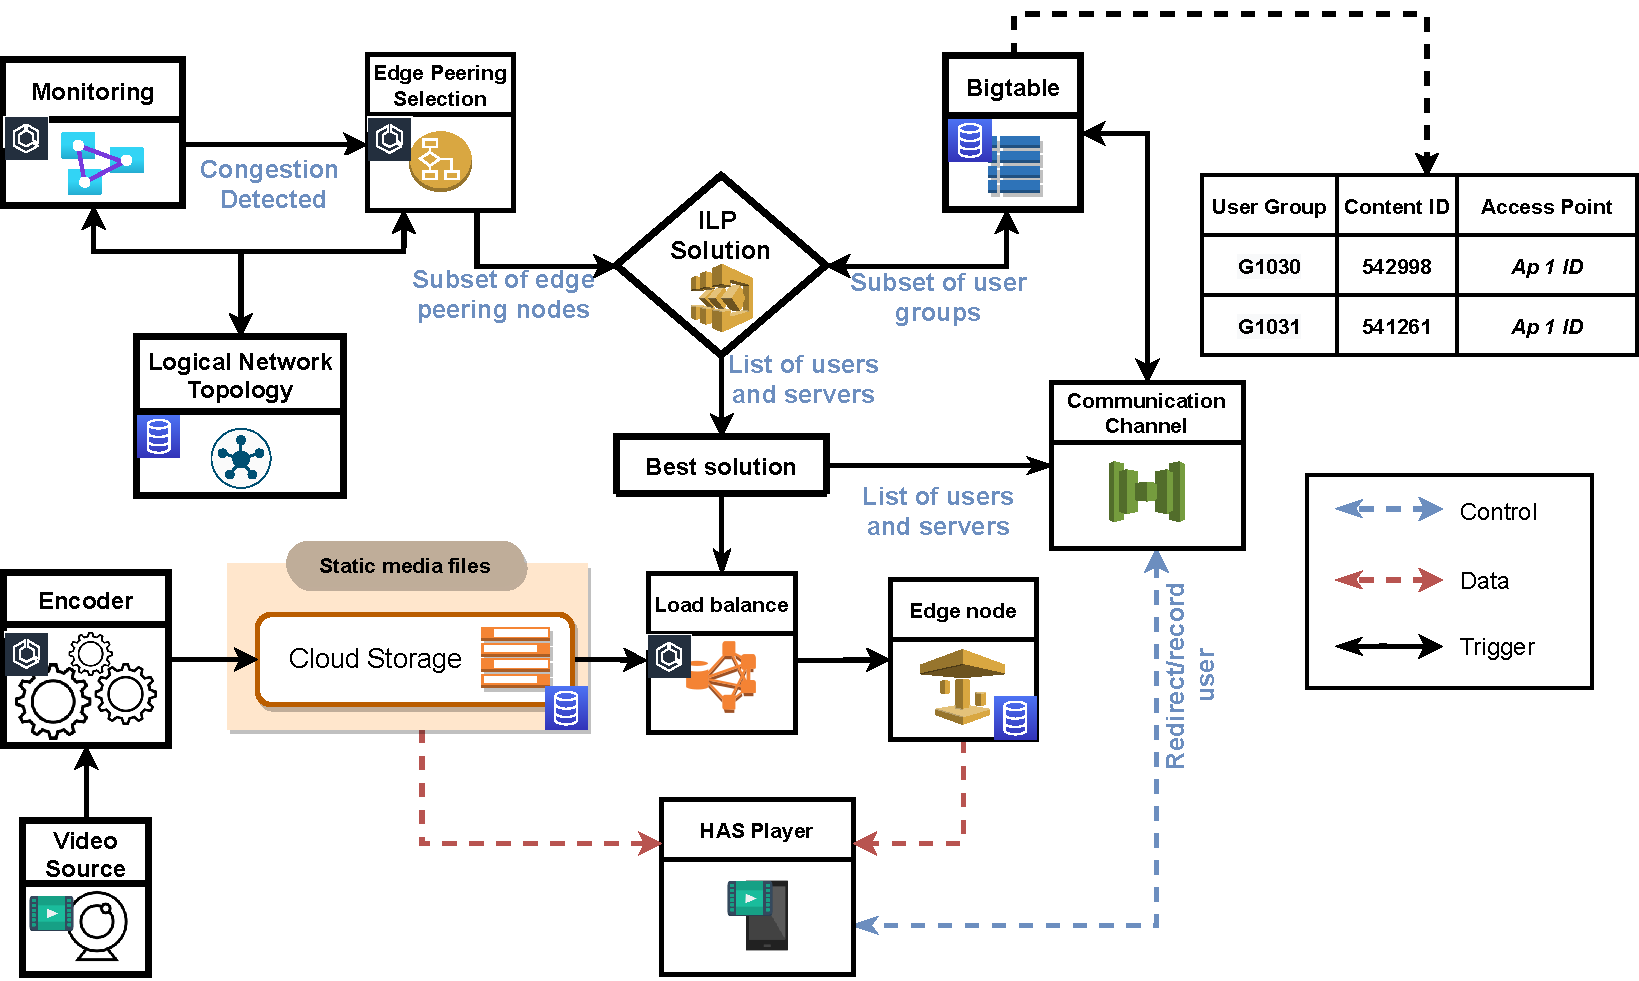
\includegraphics[width=\linewidth]{images/flow-model-infrastructure.pdf}
  \caption{Flowchart model of our proposed architecture.}
\end{figure}

Conforme ilustrado na Figura 2, apresentamos a arquitetura do sistema para realizar todas as solicitações/respostas necessárias ao serviço de streaming de vídeo. O cliente HAS primeiro solicita o manifesto ao servidor solicita o manifesto ao servidor HTTP. O reprodutor de traço solicita segmentos sequencialmente e adapta-se dinamicamente às condições da rede usando sua lógica de taxa de bits adaptável (ABR). Os esquemas ABR também levam em consideração o buffer de reprodução, recursos do dispositivo, preferências do visualizador e recursos de conteúdo. Enquanto o armazenamento em nuvem é essencialmente um servidor HTTP que armazena os pedaços de diferentes representações de vários conteúdos de vídeo e os arquivos de manifesto correspondentes.% Além dos arquivos de manifesto regulares, o servidor HAS também armazena os arquivos de manifesto de qualidade para listar as qualidades perceptivas dos pedaços. Abaixo, discutimos os componentes em mais detalhes.


\subsubsection*{Componente de Comunicação}

O Componente de Comunicação funciona como canal de controle, no qual é essencial para realizar a operação de comunicação com as redes celulares. A classe principal cria um canal de controle responsável por toda a comunicação entre as entidades. Neste trabalho são oferecidas duas funções de comunicação, \textit{i)} o redirecionamento após a execução do componente de otimização, desta forma são ativadas mensagens acionadas aos usuários no redirecionamento para outro cache de borda. Tal mensagem de redirecionamento deve ser enviada para que os usuários iniciem as requisições HTTP em um servidor já disponível. Como segunda função oferecida, \textit{ii)} informações fornecidas pelos usuários, que incluem várias variáveis de entrada (por exemplo, largura de banda disponível, nível de congestionamento, QoE, nível de buffer, resolução do dispositivo, tipo de conteúdo).
%o ID do conteúdo solicitado e dados de estado do UE (por exemplo, ocupação de buffer).
As informações também podem auxiliar o módulo de otimização com relatórios periódicos sobre aos APs disponíveis e suas intensidades de sinal.


\subsubsection*{Componente de rastreamento}

Observe que rastrear as requisições de cada usuário e direcionar as requisições a servidores de borda ou ao servidor de origem pertencem ao redirecionamento de solicitações em tempo real.

O componente de rastreamento armazena o status do player em cada etapa e acompanha os players dos usuários. Ao iniciar uma sessão de streaming, o gerenciador de requisições, primeiro, classifica o usuário em um dos grupos HAS com base em características específicas da requisição. Aqui, nós consideramos um conjunto de usuários HAS $P = \{p_1,p_2, ..., p_N\}$, onde cada usuário $p_j \in P$ é colocado dentro de um grupo de usuários. Definimos os grupos de usuários como $G_{u,b_{i}}$ que contém um subconjunto de usuários $p_j$ conectados com o mesmo AP $B(t) = \{b_{i}\}$ no momento $t$ e solicita um conteúdo de vídeo específico $u$. Depois disso, cada conjunto de jogadores que pertencem ao mesmo grupo são agregados em um nó em comum usando uma função de agregação simples (ou seja, conjunta).
Se o usuário iniciar com o pedido de manifesto a informação recebida contém o servidor atualizado, caso contrário, e o usuário já estiver visualizando o vídeo, um canal de comunicação realiza esta atualização. Ajudando assim a simplificar o processamento e a computação no componente otimizador.
% Em segundo lugar, ele formula o problema de seleção de representação como um Processo de Decisão Markov Parcialmente Observável (POMDP) com várias variáveis de entrada (por exemplo, largura de banda disponível, nível de congestionamento, QoE, nível de buffer, resolução do dispositivo, tipo de conteúdo, tipo de plano de assinatura), que representa nossa abstração do modelo POMDP consiste em três níveis, incluindo players, clusters e modelo POMDP de nível superior (agregação de todos os players). Por fim, em cada etapa, o módulo de recomendação de qualidade gerencia e armazena as decisões otimizadas por cluster resultantes do solver e, em seguida, passa essas saídas para o componente de comunicação.
Outro ponto importante é que o gerenciamento de players de usuários tende a se tornar mais fácil de manusear em um servidor centralizado, de modo que os usuários ativos são pré-organizados por este módulo.
% Isso acontece depois que o agendamento de replicação é gerado e precisa considerar a disponibilidade de conteúdo dinâmico nos servidores de borda, o que está além do escopo deste artigo.


\subsubsection*{Componente de Monitoramento}

Para decidir quando um novo nó de borda é necessário, o sistema também deve estar ciente das condições reais da rede. Portanto, um monitoramento de rede é necessário para realizar essa tarefa.
Basicamente, o componente de monitoramento tem a função de observar métricas pré-definidas da rede,neste trabalho vamos observar o consumo da largura de banda da rede. 
Consideramos um conjunto de links com largura de banda $\Lambda$, onde cada link $\lambda_{\left \langle i,j \right \rangle} \in \Lambda$ está associado a um nó de origem $i$ e destino $j$ . A estimativa de largura de banda é baseada nos pacotes recebidos/transmitidos de cada interface de rede.
%, a velocidade de download nos blocos recentes é robusta às flutuações de largura de banda. 
Periodicamente, o modulo estima a taxa de transferência de cada rede de link. Este tempo no consumo da largura de banda leva em consideração um determinado período $T$ e um estado de rede $\psi$.
%
Para estimar o \textit{throughput}, o módulo de monitoramento calcula o número de pacotes recebidos durante cada período $T$. A taxa de transferência do link atual estimada é definida como $\lambda_{\left \langle i,j \right \rangle}(\psi, t)$. A largura de banda total no link de gargalo (fixo) é representada por $\lambda^{all}_{\left \langle i,j \right \rangle}(\psi, t)$. O uso estimado do link na próxima iteração $(t+T)$ e um novo estado de rede $\psi'$ são rotulados $\lambda_{\left \langle i,j \right \rangle}(\psi', t+ T) $. Aqui, em $\psi'$ estamos considerando mudanças físicas na rede como falha de link, assim como oscilações que ocorrem ao longo do tempo, o que está além do escopo deste artigo.
% de tráfego cruzado, e assim por diante.
%Finalmente, o módulo de monitoramento usa a taxa de transferência para estimar a taxa de transferência $\lambda_{\left \langle i,j \right \rangle}(\psi, t)$ ($\leqslant \lambda^{all}_{\left \langle i,j \right \rangle}(\psi, t)$)o sistema geral deve fornecer aos usuários.


\subsubsection*{Componente de Optimização}

O objetivo do componente otimizador é decidir sobre o número de servidores capaz de atender a demanda de video, bem como distribuir os usuários entre os servidores da melhor forma. Para isso, um modelo de programação linear inteira (\textit{Integer Linear Programing} - ILP) apresentado, o modelo objetiva maximizar o o uso da infraestrutura presente de modo a satisfazer QoE dos usuários exigidas. 
Uma vez que o componente de monitoramento detecta um link congestionado, o componente otimizador é acionado. Primeiramente, o módulo de seleção de peering de borda coleta as entradas provenientes de monitoramento e bigtable, em que são um subconjunto da topologia da rede contendo os nós abaixo do link congestionado. Ao fazer isso, um subgrupo com os melhores usuários finais é selecionado dessa topologia de sub-rede.
Antes de iniciar a execução da ILP, a classe \textit{Edge Peering selection} coleta as entradas provenientes do monitoramento e, em seguida, recebe as entradas e procura maximizar o provisionamento de conteúdo de vídeo apresentado por redes multiníveis, então, uma formalização da ILP recebe a entrada e busca maximizar o provisionamento de conteúdo de vídeo apresentado por redes multinível. 
Uma vez resolvido o problema de alocação, precisamos apenas considerar o problema de replicação dentro de cada edge cluster e seus grupos de usuários atribuídos (observe que a QoE dos grupos de usuários atribuídos é garantida com alocação estável). Em seguida, formulamos o problema de replicação de cluster único considerando um determinado cluster de borda F e os grupos de usuários atribuídos a F.

% O objetivo do componente otimizador é decidir sobre o número de servidores para minimizar a escala de infraestrutura necessária, mas também maximizar o QoE dos usuários. Para isso, dividimos o tempo em duas classes principais, uma classe coleta as entradas provenientes do monitoramento, uma de programação linear inteira (ILP) recebe a entrada e busca maximizar o provisionamento de conteúdo de vídeo apresentado pelas redes multinível. % Na próxima seção, através de alguns experimentos, é possível verificar os impactos que ocorrem nos mecanismos de decisão ABR com uma topologia multinível simples.
%a provisão não apenas para atender a demanda de taxa de transferência de usuários finais em conteúdo de vídeo

\begin{table}[h!]
\centering
\begin{tabular}{|l|l|}
\hline
\multicolumn{1}{|l|}{\textbf{Notação}} & \multicolumn{1}{l|}{\textbf{Descrição}} \\ \hline \hline
Number of UE                    & \{10, 30, 50\}                      \\
\hline
MIMO system                     & SISO                                \\
\hline
RB block                        &  6, 25, 100                         \\
\hline
Radio frequency band            & 1.4MHz, 5MHz, 20MHz                 \\
\hline
% Downlink carrier frequency      & 2160MHz                             \\
% \hlinezz
% Uplink carrier frequency        & 1930MHz                             \\
% \hline
Number of eNodeBS               & \{1, 3\}                            \\
\hline
Channel model                   & Defined by 3GPP TS 36.104 Annex B.2 \\
\hline
Channel type                    & Fading channel described  by Rayleigh distribution \\
\hline
eNB  Noise Figure               & 2 dB                                \\
\hline
UE Noise Figure                 & 7 dB                                \\  
\hline
% Type of propagation environment & Urban                               \\
% \hline
eNode transmit power            & 46Bm                                \\
\hline
\end{tabular}
\caption{Resumo das principais notações.}
\label{tb:resu-notation}

\end{table}


A Tabela~\ref{tb:resu-notation} resume os parâmetros e variáveis do modelo. Em relação aos parâmetros, o conjunto de pontos de entrada de onde são gerados os pedidos é rotulado como GW; estes correspondem aos gateways de onde os clientes acessam o ambiente Fog.

Como os usuários geralmente acessam os segmentos de vídeo de uma transmissão sequencialmente, as demandas dos usuários para que os segmentos de vídeo sejam gerados na próxima janela de tempo curta podem ser estimadas aproximadamente pela audiência atual desse fluxo. Observe que em um modelo hierárquico, as camadas superiores dentro da rede de borda tendem a atingir um grande número de usuários finais.
Para aumentar o número de atendimentos de um único nó, usamos a função $\chi(\psi, j)$. Onde $\lambda_{i}$ é o número de usuários no grupo $i$ e $p_{j}$ é a probabilidade de que o nó $j$ possa fornecer um streaming de vídeo a vários usuários.

\begin{equation}\label{cost_func}
\chi(\psi, j) = n(cP_{j}) * (1 - p_{j})
\end{equation}
\vspace{.05cm}

Para um servidor de borda arbitrário $j$, ele deve ter largura de banda suficiente para servir $A_j$. Assim, a seguinte restrição deve ser colocada:

\begin{equation}
x_{ij} * d_{i}( bt_{i}^{max}) \leq Bw_{p_{ij}^{k}} \\
\end{equation}
\vspace{.05cm}

onde $bi$ é a largura de banda consumida pelo visualizador $i$ e $B_j$ é a largura de banda total do servidor de borda $j$.

Seja $s_i$ uma transmissão de video arbitrária de um canal com uma determinada taxa de bits. Indicamos os segmentos de vídeo a serem gerados por $s_i$ em $T$ como $D^T_i$ (ou seja, $D^T_i = \{ v^{t_1}_i, v^{t_2}_i, ..., v ^{t_n}_i \}$, onde $(t_1,t_2,...,t_n)$ são os timestamps dos segmentos de vídeo ($v_1,v_2, ..., v_n$) gerados em $T$, respectivamente ). Se usarmos $L_{A_j}$ para denotar o conjunto não redundante de fluxos acessados por espectadores em $A_j$, a seguinte restrição na capacidade do cache deve ser colocada:

\begin{equation}
\sum^{n}_{i=1} x_{ij} \leq M_{j}y_{j}
\end{equation}
\vspace{.05cm}

onde $M(.)$ é a função que calcula o tamanho total do cache de um determinado conjunto de segmentos de vídeo, $c_j$ denota a capacidade de cache do servidor de borda $j$.

% Seleção de Caminho e Alocação de Recursos
Para suportar os serviços de vídeo demandados pelos usuários, um caminho ótimo definido para todos os fluxos de dados deve ser encontrado resolvendo o algoritmo proposto. Denote $P_{i}$ como um conjunto de caminhos incluindo todos os caminhos candidatos para o usuário $i$ e $P_{ij}$ como um subconjunto de $P_{i}$ incluindo todos os caminhos candidatos a partir do nó $j$. Um caminho $p_{ij}^{k} \in P_{i}$ significa o \textit{k-th} fluxo de caminho $i$ começando do nó $j$ e a taxa de dados correspondente deste caminho é denotada por $r_{ ij}^{k}$ se $p_{ij}^{k}$ estiver selecionado.

Assim, o problema proposto pode ser formulado da seguinte forma.

\begin{equation} 
\begin{aligned}
\min{} \quad &
\sum^{G_u}_{i=1}\sum^{F}_{j=1} c_{ij}x_{ij} + \sum^{F}_{j=1} f_{j} y_{j} \\
%
\text{Subject to} \quad & 
\sum^{F}_{j=1} x_{ij} = 1 \text{ } \forall i \in G_u \\
&
\sum^{n}_{i=1} x_{ij} \leq M_{j}y_{j} \\
&
x_{ij} * d_{i}( bt_{i}^{max}) \leq Bw_{p_{ij}^{k}} \\
&
x_{ij} \geq 0 \\
&
y_{j} \in \{0,1\} 
\end{aligned}
\end{equation}

Onde $F$ e $G_u$ são definidos como o conjunto de servidores de borda em um determinado cluster de borda e o conjunto de visualizadores atribuídos pela alocação estável de um para vários, respectivamente, e $x_{i,j}$ é definido do seguinte modo:

\begin{equation}\label{total_capacity_loss}
x_{i,j} =
\begin{cases}
1 & \text{se o usuário } i \text{ requisita ao servidor } j \\ 
0 & \text{caso contrário }
\end{cases}
\end{equation}



% ==========================================

Na próxima seção, através de alguns experimentos, é possível verificar os impactos que ocorrem em mecanismos de decisão ABR com uma topologia multinível simples.
%a provisão não apenas para atender a demanda de taxa de transferência de usuários finais em conteúdo de vídeo

Uma vez que o componente de monitoramento detecta um link congestionado, o componente otimizador é acionado. Primeiramente, o módulo de seleção de peering de borda é responsável por reunir as entradas provenientes de monitoramento e bigtable, em que são um subconjunto da topologia da rede contendo os nós abaixo do link congestionado. Ao fazer isso, um subgrupo com os melhores usuários finais é selecionado dessa topologia de sub-rede.

Em seguida, utilizamos o conjunto de dados combinado para realizar uma solução no modelo ILP.
% Seleção de Caminho e Alocação de Recursos
Para suportar os serviços de vídeo demandados pelos usuários, um caminho ótimo definido para todos os fluxos de dados deve ser encontrado resolvendo o algoritmo proposto. Denote $P_{i}$ como um conjunto de caminhos incluindo todos os caminhos candidatos para o usuário $i$ e $P_{ij}$ como um subconjunto de $P_{i}$ incluindo todos os caminhos candidatos a partir do nó $j$. Um caminho $p_{ij}^{k} \in P_{i}$ significa o $k-th$ fluxo de caminho $i$ começando do nó $j$ e a taxa de dados correspondente deste caminho é denotada por $r_{ ij}^{k}$ se $p_{ij}^{k}$ for selecionado.

%\subsection{Solução de ILP proposta}


A estimativa da taxa de transferência usa a demanda que passa por $\widehat{s_{t+T}}$ para estimar a quantidade de taxa de transferência $D$ que o sistema geral deve fornecer aos usuários. Cada cliente tenta atingir uma qualidade alvo (maior taxa de bits de vídeo disponível) $Q$.
Além disso, introduzimos C, um coeficiente corretivo dinâmico para resolver os problemas de rede e servidor. Ele leva em consideração a taxa de bits média de vídeo $B (B < Q)$ exibida por todos os clientes que assistem ao fluxo e a taxa de falha $FR$, que é a parcela de clientes que não conseguiram obter a tempo a resposta de seu último pedido do servidor.

% As soluções de cache de conteúdo de requisições buscam minimizar o atraso médio de acesso ao conteúdo e maximizar a taxa média de requisições de conteúdo nos nós de edge cache, que nem sempre são alcançadas simultaneamente. Assim, um compromisso otimizado entre os dois objetivos é direcionado

% Curiosamente, a colocação de conteúdo e o agendamento de solicitações geralmente ocorrem em diferentes escalas de tempo: a popularidade do conteúdo geralmente varia lentamente, na escala de horas ou dias com base na medição e previsão de várias fontes; por outro lado, as decisões de agendamento de solicitações precisam se adaptar à dinâmica da localização do usuário e das condições do canal, que variam na ordem de segundos. Isso dificulta uma otimização conjunta para reagir prontamente às mudanças dinâmicas da rede; portanto, motiva a decomposição do problema geral em (i) o subproblema de gerenciamento de cache, que leva a popularidade do conteúdo a longo prazo como entrada, e (ii) o subproblema de escalonamento de solicitação de conteúdo, que leva em consideração as solicitações específicas recebidas, a condição de canal correspondente dos usuários e a disponibilidade de cache nas BSs e na CPU. Embora os dois subproblemas sejam tratados separadamente devido às suas diferentes escalas de tempo, o acoplamento entre os dois se reflete no fato de que a solução da política de colocação de cache é usada como entrada para a política de agendamento de requisições. Da mesma forma, a solução de agendamento de solicitações afetará a decisão de colocação de cache na próxima vez que for recalculada. Isso ocorre porque a popularidade do conteúdo é calculada com base no número de solicitações para cada conteúdo em diferentes BSs como resultado da política de agendamento de solicitações; portanto, após um longo período de escala de tempo (horas ou dias), a decisão de colocação do cache será feita com base na popularidade do conteúdo atualizado

% \subsection{Management Mechanism}

% Neste trabalho, o cliente e o servidor utilizam o protocolo HTTP na camada de aplicação para realizar todas as requisições/respostas necessárias. No lado do servidor, uma vez que um arquivo de mídia ~ (ou fluxo) esteja pronto, ele será preparado para streaming antes de ser publicado em um servidor HTTP padrão. O arquivo/stream original é particionado em segmentos~(também chamados \textit{chunks}) de tempo de reprodução equivalente, e várias versões (também chamadas de representações) de cada segmento são geradas que variam em taxa de bits/resolução/qualidade usando um codificador ou um transcodificador .
% Além disso, o servidor gera um arquivo de manifesto chamado descritor de apresentação de mídia~(MPD), que lista as representações disponíveis, incluindo informações como tempo de vídeo, disponibilidade de conteúdo, tipos de mídia~(ou seja, H.264 , H.265, etc. .), resoluções, larguras de banda mínimas e máximas, e a existência de várias alternativas codificadas de componentes multimídia, localização de segmentos de mídia na rede e outras características de conteúdo.

% No lado do cliente HAS, primeiro, o player de vídeo solicita o manifesto ao servidor HTTP e analisa as informações mencionadas acima. Dessa forma, ele pode começar a solicitar segmentos sequencialmente e adaptar-se dinamicamente às condições da rede usando sua lógica adaptativa de taxa de bits~(ABR). Os esquemas ABR também levam em consideração o buffer de reprodução, recursos do dispositivo, preferências do visualizador, bem como recursos de conteúdo, com pesos diferentes.
% Como a QoE do espectador precisa ser determinada em tempo real durante a reprodução, métricas objetivas são frequentemente usadas, incluindo o número de interrupções, duração do atraso de inicialização, frequência e número de oscilações de qualidade de vídeo. Por padrão, o HAS não requer nenhum esquema de adaptação específico, deixando os desenvolvedores de sistemas inovarem e implementarem seus próprios métodos.

% O controlador dentro do servidor CDN possui um canal de comunicação é criado com o usuário, assim as nossas mecanismos são capazes de se adaptar em tempo-real as necessidades da rede, bem como melhorar as

% \begin{algorithm} \caption{Mecanismo de gerenciamento multimídia em tempo real}
% \begin{algorithmic}[1]

% % \State Initilize $V(s) = 0$, for all $s \in \mathcal S^+$

% \State /* Phase 1: Make Decision related to the cache allocation and media content. */
% \State Initialize $a_i = 0$, for all viewer $i \in M$;
% \For {$i \in \textit{Grupos de usuários}$}
%     \State $j \leftarrow \textup{head of } S_{i}$;
%     \State Insert $i$ into $G_{j}$~($G_{j}^{k \cup i}$);
%     \If{$D(G_{j}^{0 \sim k}) \leq C_{j}$}
%         \State Label $G_{j}^{0 \sim k}$ with $j$;
%     \EndIf
%     % \State $v \gets V(s)$
%     % \State $V(s) \gets \sum_a \pi(s,a) \sum_{s'} \mathcal P_{ss'}^a [ \mathcal R_{ss'}^a + \gamma V(s')$
%     % \State $\Delta \gets \max(\Delta, |v- V(s)|)$
% \EndFor

% \State /* Phase 2: Redirecting viewers. */
% \For{viewer i with ai = 0}
%     \If{\textit{exists server} $j \in F$ \textit{with} $bd_j \geq b_i$ \textit{•}it{and} $s_i \in S_j$} 
%         \State $a_i \gets j$; $bd_j \gets (bd_j - b_i)$;
%     \EndIf 
% \EndFor

% \State /* Phase 3: Offload Media Content tasks. */

% \Ensure $S_i$
% \end{algorithmic}
% \end{algorithm}
